\documentclass[11pt,a4paper,landscape,fleqn]{article}
\usepackage[utf8]{inputenc}
\usepackage[english]{babel}
\usepackage{multicol}
\usepackage[margin=0.5in]{geometry}
\usepackage{amsmath}
\usepackage{amssymb}
\usepackage{enumerate}
\usepackage{fancyhdr}
\usepackage{graphicx}
\usepackage{wrapfig}


\graphicspath{ {./images/} }

\everymath{\displaystyle}
\pagestyle{fancy}
\fancyhf{}

\setlength{\mathindent}{0pt}
\renewcommand{\headrulewidth}{0pt}
\renewcommand{\footrulewidth}{2pt}

\lfoot{\bfseries Prashant Dhirendra : prashant.dhiru@gmail.com} 
\begin{document}
\begin{multicols*}{3}
{\noindent \bfseries {\Large Trigonomartric Basics}}\\ \\
$\pi^r = 180^{\circ}$\\ \\
$\sin\theta = \frac{1}{\csc\theta} = \frac{P}{H}$\\ \\
$\cos\theta = \frac{1}{\sec\theta} = \frac{B}{H}$\\ \\
$\tan\theta = \frac{1}{\cot\theta} = \frac{P}{B}$\\ \\ 
{\bfseries {Identities}}\\ \\
$\sin^2\theta+ cos^2\theta = 1$\\
$1 + \tan^2\theta = \sec^2\theta$ \\
$1 + \cot^2\theta = \csc^2\theta$ \\ \\
{\indent $\sec\theta + \tan\theta = \frac{1}{\sec\theta - \tan\theta}$}\\ \\
{\indent $\csc\theta + \cot\theta = \frac{1}{\csc\theta - \cot\theta}$}\\ \\
{\bfseries {Angle}}\\
for $ < 360 \quad 580 = (580-360)=220$\\
Aaja Sanam Teri Cosam(ASTC)\\
{\bfseries {Allied Angle}}\\
\begin{center}
\begin{tabular}{|| c| c|| }
\hline
$180 \pm \theta$ & $90 \pm \theta$\\
$260 \pm \theta$ & $ 270 \pm \theta$\\[0.5 ex]
\hline
$\sin \rightarrow \sin$   &  $\sin \leftrightarrow \cos$\\
$\cos \rightarrow \cos$ & $\tan \leftrightarrow \cot $\\
$\tan \rightarrow \tan$ & $\sec \leftrightarrow \csc$\\
\hline
\end{tabular}
\end{center}
$+/-$ depents on original angle\\ \\
{\bfseries {tan and cot $90^\circ-\theta$}}\\
$\tan\theta \tan(90-\theta) = 1$\\
$\cot\theta \cot(90-\theta) = 1$
\vfill\null
\columnbreak
{\bfseries {Min/Max Value}}\\
$-1 \leqslant  \sin\theta / \cos\theta \leqslant 1$\\
$-\infty \leq  \tan\theta / \cot\theta \leq \infty$\\
$-1 \geqslant \sec\theta / \csc\theta \geqslant 1$\\ \\
$ 0 \leqslant \sin^2\theta/ \cos^2\theta \leqslant 1$ \\ \\
{\bfseries {For eq : $a\sin\theta + b\cos\theta$}}\\
min/ max : $\pm \sqrt{a^2 + b^2} $\\ \\
{\bfseries {-ve angles}}\\
$\sin(-\theta) = - \sin\theta$\\
$\cos(-\theta) = \cos\theta$\\
$\tan(-\theta) = -\tan\theta$\\
NOTE : same for reciprocal \\ \\
{\noindent \bfseries {\Large Trigonometry in Geometry}}\\
$\rule{\columnwidth}{1pt}$
{\bfseries {Area of Triangle}}\\
\begin{wrapfigure}{l}{0.3\linewidth}
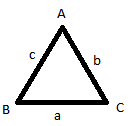
\includegraphics [scale=.6]{geo1}
\end{wrapfigure}
area $ = \frac{1}{2}bc \sin A$ \\ \\
area $ = \frac{1}{2}ac \sin B$ \\ \\
area $ = \frac{1}{2}ab \sin C$ \\ \\  \\
{\bfseries {Sin Rules}}
$$\frac{a}{\sin A} = \frac{b}{\sin B} = \frac{c}{\sin C}= 2R$$
{\bfseries {Cos Rules}} : \{Similar for A B C \}
$$\cos A = \frac{b^2+c^2-a^2}{2bc}$$
$\rule{\columnwidth}{1pt}$
\vfill\null
\columnbreak
\begin{wrapfigure}{l}{0.1\columnwidth}
\centering
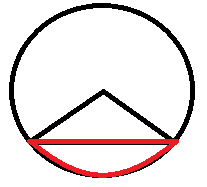
\includegraphics [scale=.4]{geo2}
\end{wrapfigure}
\hspace{5mm}{\bfseries {Length of Segment}}
$$\frac{2\pi r\theta}{360^{\circ}}+{2r\sin(\theta/2)}$$
\\ \\
{\bfseries {Area of parlleogram}} : $ab\sin\theta$\\
$\rule{\columnwidth}{1pt}$
{\bfseries {Sum and Difference of Angles}}\\
$\sin(A+B) = \sin A \cos B + \cos A \sin B$\\
$\cos(A+B) = \cos A \cos B - \sin A \sin B$\\ \\
$\tan(A+B) = \frac{\tan A + \tan B}{1 - \tan A \tan B}$\\ \\
$\cot(A+B) =\frac{\cot A \cot B -1}{\cot B + \cot A}$\\ \\
{\bfseries {Double Angle}}
\begin{flalign*}
\sin (2A) & = 2\sin A \cos A\\
& = \frac{2\tan A}{1 + \tan^2A }\\ \\
\cos (2A) & = \cos^2 A + \sin^2 A\\
& = 1 - 2\sin^2 A\\
& = 2\cos^2 A -1\\
&= \frac{1-\tan^2 A}{1+\tan^2 A}\\ \\
\tan (2A) & = \frac{2\tan A}{1-\tan^2 A}
\end{flalign*}
{\bfseries {Triple Angle}}
\begin{align*}
\sin (3x)  &= 3\sin x - 4\sin^3x\\
\cos (3x)  &= 4\cos^3x - 3\cos x\\
\tan (3A)  &= \frac{3\tan x - \tan^3x}{1-3\tan^2 x}
\end{align*}
\vfill\null
\columnbreak
{\bfseries \noindent {Value of some angle}}\\
\begin{center}
\begin{tabular}{||c|| c c c c c||}
\hline
&0 or $2\pi$ &$\pi/6$ &$\pi/4$ &$\pi/3$ &$\pi/2$\\ [1ex]
& 0 & 30 & 45 & 60 & 90\\
\hline \hline
$\sin\theta$ & 0 & $\frac{1}{2}$ & $\frac{1}{\sqrt2}$& $\frac{\sqrt3}{2}$& $1$\\ 
$\cos\theta$ & 1 & $\frac{\sqrt3}{2}$ & $\frac{1}{\sqrt2}$& $\frac{1}{2}$& $0$\\ 
$\tan\theta$ & 0 & $\frac{1}{\sqrt3}$ & $1$& $\sqrt3$& $N.D$\\
\hline
\end{tabular}
\end{center}
{\bfseries \noindent {Sum into Product}}
\begin{align*}
\sin x + \sin y &=&2 & \sin \frac{x+y}{2} &\cos\frac{x-y}{2}\\
\sin x - \sin y &=&2  & \sin \frac{x-y}{2} &\cos \frac{x+y}{2}\\
\cos x + \cos y &=+ &2 & \cos \frac{x+y}{2} &\cos \frac{x-y}{2}\\
\cos x - \cos y &= -&2 & \sin \frac{x+y}{2} &\sin \frac{x-y}{2}\\
\tan x \pm \tan y &=&& \frac{\sin(x\pm y)}{\cos x \cos y}
\end{align*}
{\bfseries \noindent {Product into Sum}}
\begin{align*}
2\sin x \cos y &= \sin(x+y)+\sin(x-y)\\
2\cos x \sin y &= \sin(x+y) - \sin(x-y)\\
2\cos x \cos y &= \cos(x+y) + \cos(x+y)\\
2\sin x \sin y &=  \cos(x-y) - \cos(x+y) 
\end{align*}
{\bfseries \noindent {$60^\circ$ Formula}}
\begin{align*}
\sin x \sin (60-x) \sin (60+x) &= \frac{1}{4}\sin 3x\\ \\
\cos x \cos(60-x) \cos(60+x)&= \frac{1}{4}\cos 3x\\ \\
\tan x \tan(60-x) \tan(60+x)&= \tan 3x
\end{align*}

\end{multicols*}
\end{document}